%!TEX root =  ../main.tex

\objective{Use but also know the limitations of inverse trigonometric functions}


The standard trigonometric functions work by receiving angles as input, and outputting
the appropriate ration of side from the Unit Circle.  Often, we need have the ratio of sides
and wish to know the angle that must exist between them.  Thinking in terms of functions,
this is the inverse of the normal, asking for the input corresponding to a given output.
But as we saw last section, the trigonometric functions all have an infinite number of
repetitions of each output.  They are not invertible.

That is to say, they do not invert to functions across their entire domains.  We must limit
their possible input if their inverses are to be functions.  The criteria of deciding the
inverse domains are:
\begin{itemize}
\item All possible outputs must be represented
\item Be as continuous as possible
\item Be centered around the origin
\end{itemize}

insert 6 inverse relations and highlighted ranges

insert unit circle with relevant semi-circles

\subsection{Composing}
\subsubsection{Inverse inside Normal}
It is straight-forward to interpret $\sin(\sin^{-1}(\frac{1}{2}))$:  ``What is sine when
sine is one-half?''  Very easy: it is one-half!  What about $\sin(\cos^{-1}(\frac{1}{2}))$?
``What is sine, when cosine is one-half?''  We could fine the angle were cosine has that
value ($60^\circ$) and take the sine of that angle, but we could also recognize that
arccosine is giving us adjacent-over-hypotenuse, and sine is asking for opposite-over-hypotenuse,
and easy problem to solve with Pythagorus's help.  It is $\frac{\sqrt{3}}{2}$.

The second approach --- drawing a right triangle with two of the side-lengths known --- is
a much more power tool and extendable to more circumstances.  Consider 
$\cos(\sin^{-1}(x))$.  ``What is cosine when sine is $x$?''  Again, sine is giving us
adjacent over hypotenuse.  We can imagine a right-triangle with one angle, call it
$\theta$.  Sine of $\theta$ means the adjacent is $x$ and the hypotenuse is 1.
The Pythagorean Theorem will allow is to find the opposite: it must be $\sqrt{1-x^2}$.

\begin{figure}
\begin{centering}
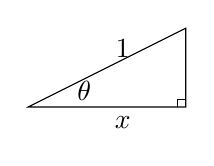
\begin{tikzpicture}
	\draw (0,0) -- (2,0) -- (2,1) -- cycle;
	\node (A) at (1.2,0) [anchor=north] {$x$};
	\node (B) at (1.2,.5) [anchor=south] {1};
	\node (C) at (.5,.2) [anchor=west] {$\theta$};
	\draw (1.9,0) -- (1.9,.1) -- (2.0,.1);
\end{tikzpicture}
\caption{A visualization of $\cos(\sin^{-1}(x))$.}
\end{centering}
\end{figure}

\subsubsection{Normal inside Inverse}
Perhaps you would be surprised at the answer if you put $\sin^{-1}(\sin(3))$ into your
TI-8*.  Would you expect it to answer 3?  How can we verbalize what this expression
is asking?  ``Extend an arc 2 units and record the resulting height above the $x$-axis.
What angle produces this height above the $x$-axis?''  We could interpret it visually
on the unit circle like this:

\begin{figure}[h]
\begin{centering}
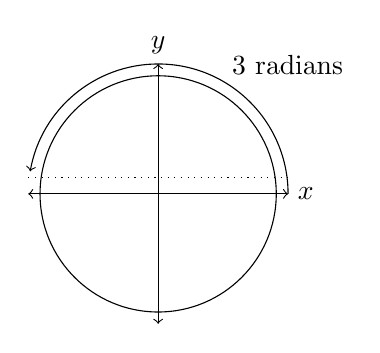
\begin{tikzpicture}[scale=1.5]
	\draw[<->] (-1.1,0) -- (1.1,0) node [anchor=west] {$x$};
	\draw[<->] (0,-1.1) -- (0,1.1) node[anchor=south] {$y$};
	\draw (0,0) circle (1);
	\draw[->] (0,0) ++ (0:1.1) arc (0:170:1.1) node[midway,xshift=1.5cm] {3 radians};
	\draw[dotted] (-1.1,0.14) -- (1.1,0.14);
\end{tikzpicture}
\caption{3 radians is a height arcsine can find in \texttt{QI}.}
\end{centering}
\end{figure}

Notice that the height above the $x$-axis -- the sine of the angle -- is achievable in
the first quadrant.  Arcsine --- because it is a function and can only return one
value per input --- must answer a positive input in the first quadrant.

\subsection{Derivatives}
How can we find the derivatives of inverse trigonometric functions?  The
definitions of inverses is very helpful: swapping $x$ and $y$.  Inverse sine is just
$x=\sin(y)$.  Using implicit differentiation, we get $dx=\cos(y)dy$.  Therefore,
$$
\frac{dy}{dx} = \frac{1}{\cos(y)} = \frac{1}{\cos(\sin^{-1}(x))}
$$

As we saw above, this can be simplified.  You will find all six inverse trigonometric 
functions derivatives in the exercises.
